\documentclass[final]{ukthesis}
%you must include these 2 packages.
\usepackage{setspace}
\usepackage{float}
\usepackage{memhfixc}
\usepackage{graphicx}
\usepackage{amssymb,amsmath}
\usepackage{caption}
\usepackage{tabularx}
\usepackage{cite}
\usepackage{bm}
\usepackage{url}
\usepackage{upgreek}
\usepackage{subcaption} 
\usepackage[perpage]{footmisc}
\usepackage{braket}
\usepackage[numbers]{natbib}
\usepackage{etoolbox}
\usepackage[pdfauthor={Michael Brown},
            pdftitle={The Title},
            pdfsubject={The Subject},
            pdfkeywords={Some Keywords},
            pdfproducer={Latex with hyperref},
            pdfcreator={latex->dvips->ps2pdf},
            pdfpagemode=UseOutlines,
            bookmarksopen=true,
            letterpaper,
            bookmarksnumbered=true,
            backref=page,
            hyperfootnotes=true]{hyperref}
\makeatletter
\patchcmd{\BR@backref}{\newblock}{\newblock(page~}{}{}
\patchcmd{\BR@backref}{\par}{)\par}{}{}
\makeatother


\newcolumntype{M}[1]{>{\centering\arraybackslash}m{#1}}
\newcolumntype{N}{@{}m{0pt}@{}}

\changetocdepth{3}
\maxsecnumdepth{subsection}
\maxsecnumdepth{subsubsection}

\usepackage{titlesec}
\titleformat{\chapter}[display]
  {\bfseries\huge}
  {\filleft\Large\chaptertitlename~\thechapter}
  {2.5ex}
  {{\titlerule[1.0pt]}\vspace{1.0ex}\filright}
  [\vspace{1.0ex}{\titlerule[1.0pt]}]

\titleformat*{\section}{\large\bfseries}
\titleformat*{\subsection}{\normalsize\bfseries}
\titleformat*{\subsubsection}{\small\bfseries}

\usepackage{xcolor}
\hypersetup{
    colorlinks,
    linkcolor={red!50!black},
    citecolor={blue!50!black},
    urlcolor={blue!80!black}
}

\usepackage{ntheorem}
\newtheorem{theorem}{}
\newtheorem*{theorem-non}{}

%\usepackage{fleqn}
%\setlength{\mathindent}{30.0pt}

\newlength{\figwidth}
\setlength{\figwidth}{\textwidth}
\sloppy
%%%%%%%%%%%%%%%%%%%%%%%%%%%%%%%%%%%%%%%%%%%%%%%%
\begin{document}
%author data

\author{Michael Brown}

\title{UCNA Experiment: Analysis of 2011/2012 and 2012/2013 Data Sets}

\abstract{
The UCNA Experiment at the Los Alamos Neutron Science Center (LANSCE) is the first measurement  of the $\beta$-decay asymmetry parameter $A_0$ using polarized ultracold neutrons (UCN). $A_0$, which represents the parity-violating angular correlation between the direction of the initial neutron spin and the emitted decay electron's momentum, determines $\lambda=g_{A}/g_{V}$, the ratio of the weak axial-vector and vector coupling constants. A high-precision determination of $\lambda$ is important for weak interaction physics, and when combined with the neutron lifetime it permits an extraction of the CKM matrix element $V_{ud}$ solely from neutron decay. At LANSCE, UCN are produced in a pulsed, spallation driven solid deuterium source and then polarized via transport through a 7 T magnetic field. Their spins can then be flipped via transport through an Adiabatic Fast Passage spin flipper located in a low-field-gradient 1 T field region prior to transport to a decay storage volume situated within a 1 T solenoidal spectrometer. Electron detector packages located at each end provide for the measurement of decay electrons. Previous UCNA results (based on data collected in 2010 and earlier) were limited by systematic uncertainties, in particular those from the UCN polarization, calibration of the electron energy, and electron backscattering. This dissertation will present a background of Neutron Decay, an overview of the UCNA Experiment, followed by a detailed report on the entire analysis process for the 2011/2012 and 2012/2013 data sets.
}

\advisor{Dr. Bradley Plaster}
\keywords{BLAH BLAH}
\dgs{Dr. Tim Gorringe}
%the title pages
\frontmatter
\maketitle

\begin{dedication}
  This work is dedicated to my parents, Cindy and John, and my soon-to-be wife, Kirstie, for their
  unending support. And also to Piper, my four-legged friend who keeps me sane.
\end{dedication}

\begin{acknowledgments}
  The friendship and guidance provided by Dr. Brad Plaster made this work possible. I thank you.
  Also to Dr. Renee Fatemi, Dr. Susan Gardner, and Dr. Kevin Donohue, I thank you for serving on
  my dissertation committee and seeing this process through.
\end{acknowledgments}


\tableofcontents\clearpage
\listoffigures\clearpage
\listoftables\clearpage
%----------------------------------------------
\mainmatter
\DoubleSpacing

\chapter{Introduction}
\label{ch:Introduction}

The purpose of this dissertation is to describe in detail
the methods used in extracting the $\beta$-decay asymmetry parameter
for the UCNA Experiment. This chapter hopes to motivate the inception
of the parameter of interest and its role in the theory of $\beta$-decay.
Also introduced are characteristics of the neutron itself with an
emphasis on ultracold neutrons (UCN), the namesake of the UCNA experiment.

%%%%%%%%%%%%%%%%%%%%%%%%%%%%%%%%%%%%%%%%%%%%%%%%%%%%%%%%%%%%%%%%%%%%%%%%%%%%%%%
%%%%%%%%%%%%%%%%%%%%%%%%%%%%%%%%%%%%%%%%%%%%%%%%%%%%%%%%%%%%%%%%%%%%%%%%%%%%%%%

\section{The Standard Model}
The Standard Model of particle physics encompasses everything we know about
interactions between particles and describes nature using the most fundamental
building blocks yet discovered. This section is used as an introduction
to these building blocks, the quarks and leptons, and to the mediators of the
interactions between them, to preface the upcoming descriptions of the neutron
and $\beta$-decay.

\subsection{The Building Blocks}

\subsection{The Forces}

\subsection{Symmetries}



%%%%%%%%%%%%%%%%%%%%%%%%%%%%%%%%%%%%%%%%%%%%%%%%%%%%%%%%%%%%%%%%%%%%%%%%%%%%%%%
%%%%%%%%%%%%%%%%%%%%%%%%%%%%%%%%%%%%%%%%%%%%%%%%%%%%%%%%%%%%%%%%%%%%%%%%%%%%%%%

\section{Properties of the neutron}
\label{sec:neutronProperties}
Let us take a moment to give a very brief introduction to the neutron to motivate the
upcoming sections. This will also serve as a useful tool for those who are
unfamiliar with nuclear and field theories, as the following sections become
quite technical. The majority of this dissertation can be read and mostly understood
without much knowledge of the theoretical description behind neutron $\beta$-decay,
so the properties of the neutron are a natural starting point.

The neutron is a net neutrally charged composite particle. The terms net and
composite hint at the inner structure of the neutron, made up of fundamental
particles called quarks, in this case two down ($d$) quarks and one up ($u$) quark.
The quarks do carry charge, with the $u$ charge $+2/3$ and the $d$ charge
$-1/3$, so that the net charge of the neutron is zero. This can be compared
to the proton, another composite particle made up of three quarks (two $u$ and
one $d$ quark), whose net charge is $+1$ and the other nucleon found
within a nucleaus along with the neutron. Four other quarks exist,
the charm, strange, bottom, and top in order of increasing mass. The neutron
is the second lightest three-quark composite particle (baryon) 
behind only the proton.

The free neutron undergoes $\beta$-decay, defined as a transition from the neutron
to a proton, electron, and electron anti-neutrino,
\begin{equation*}
  n\rightarrow p + e^- + \bar{\nu}_{e}.
\end{equation*}
\noindent The three-body decay gives rise to a continuous energy spectrum
for the proton, electron, and anti-neutrino by conservation of energy and momentum
as seen in figure \ref{fig:spectralShapes}. The lifetime of the free neutron is
approximately fifteen minutes.


\section{$\beta$-decay of the neutron}

Prior to 1930, $\beta$-decay of nuclei was a polarizing topic of debate. Originally
only the decay electron was detected, and given such a two-body decay (the recoil
nucleus and the emitted electron being the two bodies) one would expect a discrete
electron energy defined by the difference in mass between mother and daughter
nuclei. Instead, a continuous energy spectrum was observed for the electron, which
initially led some to believe that energy conservation was moot. Others, like
Wolfgang Pauli, were not ready
to abandon energy conservation. He postulated that a neutral particle
could also be emitted in the decay. This third particle would share the energy available
in the reaction, explain the continuous energy distribution of the electron, and go
on undetected as it would not interact electromagnetically. The particle was termed
the neutrino by Fermi, and it would be a crux of Fermi's theory of $\beta$-decay.
A quarter century later, the existence of the neutrino would be confirmed
experimentally \cite{cowan1956detection}.

\subsection{Fermi's Theory of $\beta$-decay}
After Pauli postulated the existence of the neutrino to explain the continuous energy
distribution of the $\beta$-decay electron, Fermi attempted to theoretically describe
the process in a similar manner to the theory of emission of
gamma radiation from an excited nucleus \cite{fermi1934,wilson1968fermi}.
His theory relied on two postulates: the existence of the neutrino and that the nucleus consisted
of heavy particles only, the neutron and the proton, both of which would turn out to be true.

\begin{table}[h]
  \caption{Transformation behavior of all possible bilinear covariants.} 
  \centering
  \begin{tabular}{l c }
    \hline \hline \\ [-1.75ex]
    $\bar{\psi}\psi$ & scalar \\ [0.50ex]
    $\bar{\psi}\gamma^5\psi$ & pseudoscalar \\ [0.50ex]
    $\bar{\psi}\gamma^{\mu}\psi$ & vector \\ [0.50ex]
    $\bar{\psi}\gamma^{\mu}\gamma^5\psi$ & axial vector \\ [0.50ex]
    $\bar{\psi}\sigma^{\mu\nu}\psi$ & antisymmetric tensor \\ [0.50ex]   
    \hline
  \end{tabular}
  \label{tab:bilinearCov}
\end{table}

Fermi's Hamiltonian took the form (written in a different manner from Fermi's original
paper on the subject for the sake of clarity) 
%
\begin{equation}
  H = C_V\big( \bar{\psi}_p \gamma_\mu \psi_n \big) \big( \bar{\psi}_e \gamma^\mu \psi_\nu \big), 
\end{equation}
%
where $\bar{\psi} \gamma_\mu \psi$ is a vector current (see table \ref{tab:bilinearCov}). The assumption
that the current-current interaction would be of the vector-vector variety was a natural
choice as this is the case for electromagnetism.

\begin{figure}
  \centering
  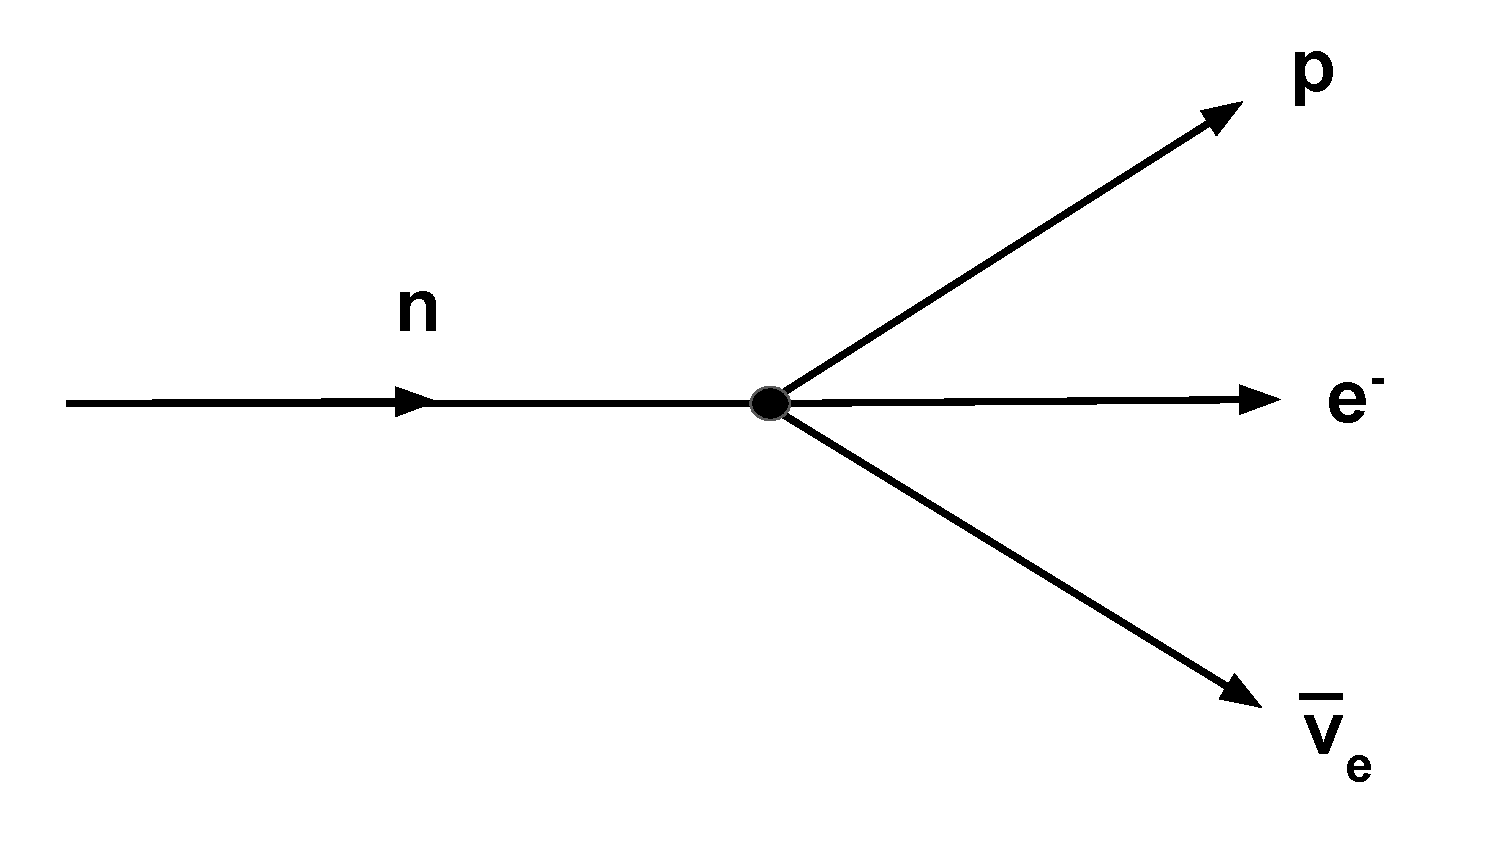
\includegraphics[scale=0.50]{1-Introduction/pointInteraction.pdf}  
  \caption{The point interaction of Fermi's theory of $\beta$-decay. The theory is
    capable of describing other processes which move one of the outgoing particle lines
    to the left side, like electron capture by the proton producing a neutron and an
    electron neutrino.}
  \label{fig:pointInteraction}
\end{figure}

Fermi's theory of $\beta$-decay treats the decay as a four-point contact interaction
(see figure \ref{fig:pointInteraction}), where
the currents are evaluated at the same point in space and time \cite{renton1990}. For those
familiar with quantum field theory within the Standard Model, this differs from the typical
interaction Hamiltonian as there is no propagator, or force carrier, to mediate the
interaction between the two currents (more on this later). The theory
worked well at predicting the energy spectrum of the electron from which
Fermi deduced that the neutrino must be nearly massless, but suffered one flaw. The vector
nature of the theory did not permit the observed allowed nuclear $\beta$-decay transitions
which can transform the spin of the decaying nucleus. This was pointed out by Gamow and Teller in
1936 \cite{gamow1936}, where they show that a current-current interaction that transforms like
a pseudovector properly assigns the spins of the products in thorium decays. As such,
one can generalize Fermi's theory by including all possible bilinear covariant terms that
satisfy both Lorentz and translational invariance:
%
\begin{multline}
  H = C_S\big( \bar{\psi}_p \psi_n \big) \big( \bar{\psi}_e  \psi_\nu \big) 
  +C_V\big( \bar{\psi}_p \gamma_\mu \psi_n \big) \big( \bar{\psi}_e \gamma^\mu \psi_\nu \big) \\
  +C_T\big( \bar{\psi}_p \sigma^{\mu\nu} \psi_n \big) \big( \bar{\psi}_e \sigma^{\mu\nu} \psi_\nu \big) 
  +C_A\big( \bar{\psi}_p \gamma_\mu \gamma^5 \psi_n \big) \big( \bar{\psi}_e \gamma^\mu \gamma^5 \psi_\nu \big) 
  +C_P\big( \bar{\psi}_p  \gamma^5 \psi_n \big) \big( \bar{\psi}_e  \gamma^5 \psi_\nu \big),
\end{multline}
%
where the coefficients quantify the coupling to each respective current.

This shortcoming of Fermi's original vector-vector interaction
lends itself to the definition of
two types of allowed $\beta$-decay transitions. The Fermi transition proceeds through the
scalar and vector currents with $\Delta J=0$ and no parity change. Gamow-Teller transitions
correspond to the axial vector and tensor currents and have $\Delta J=0,\pm1$ with no parity change,
but excluding the $0^+\rightarrow 0^+$ nuclear transitions. The pseudoscalar terms does not
contribute to the amplitude in the low energy limit \cite{renton1990}.
 

\subsection{Parity Violation in Weak Decays}

\subsubsection{Lee and Yang}

Prior to the 1950's, all discrete symmetries (parity, charge conjugation, and time reversal)
were thought to be conserved separately for all interactions in nature. A dilemma arose when
two particles, called the $\tau$ and $\theta$ mesons at the time, posessed the same mass
and charge as the $K^+$ meson, but decayed to different final states of parity. The $\tau$ decayed into three pions
and the $\theta$ into two pions. The initial classification of the two observably identical particles into
two different particles was logical given that parity conservation was then sacrosanct,
but in 1956 Lee and Yang proposed a very different solution to the problem. They realized that
there was no evidence that parity must be conserved in the weak interaction.
In the full expression of Fermi's theory (equation \ref{eq:FermiFull}),
while including all possible combinations of bilinear covariants, there was no mixing between the
individual currents and each individual current-current term transforms like a scalar. For example,
two individual axial vector currents would each transform as
$P(\bar{\psi}_p \gamma_\mu \gamma^5 \psi_n) \rightarrow -\bar{\psi}_p \gamma_\mu \gamma^5 \psi_n$ under parity, but the
muliplication of two such terms transforms like a scalar. Thus, none of the terms in \ref{eq:FermiFull})
are capable of violating parity, as the Hamiltonian would remain invariant. 

In their 1956 paper \cite{leeyang1956}, Lee and Yang modified the weak ineraction Hamiltonian
by including the possibility of a pseudoscalar current-current interaction, namely
%
\begin{multline}
  H = \bar{\psi}_p \psi_n \big( C_S\bar{\psi}_e  \psi_\nu + C'_S\bar{\psi}_e \gamma^5 \psi_\nu \big) \\
  + \bar{\psi}_p \gamma_\mu \psi_n  \big( C_V\bar{\psi}_e \gamma^\mu \psi_\nu + C'_V\bar{\psi}_e \gamma^\mu \gamma^5 \psi_\nu \big) 
  + \bar{\psi}_p \sigma^{\mu\nu} \psi_n \big( C_T\bar{\psi}_e \sigma^{\mu\nu} \psi_\nu + C'_T\bar{\psi}_e \sigma^{\mu\nu} \gamma^5 \psi_\nu \big)\\
  + \bar{\psi}_p \gamma_\mu \gamma^5 \psi_n \big( C_A\bar{\psi}_e \gamma^\mu \gamma^5 \psi_\nu + C'_A\bar{\psi}_e \gamma^\mu \psi_\nu \big) 
  + \bar{\psi}_p  \gamma^5 \psi_n \big( C_P\bar{\psi}_e  \gamma^5 \psi_\nu + C'_P\bar{\psi}_e \psi_\nu \big).
  \label{eq:leeyang}
\end{multline}
%
If any of the $C'_i$ coefficents are nonzero, parity would not be conserved due to
the scalar-pseudoscalar form of the current-current interactions that are labelled by
the primed coefficients.

Along with the inclusion of potential parity violating terms in the Hamiltonian, Lee and Yang
presented several potential tests of parity violation in the weak sector. One such proposition
was the measurement of the correlation between the spin of a polarized nucleus and
the momentum of the $\beta$-decay electron.

\subsubsection{Discovery of Parity Violation}

Following the publication of Lee and Yang's newly modified theory of $\beta$-decay, C. S. Wu
and collaborators designed an experiment \cite{wu1957} to test the potential violation
of parity in the $\beta$-decay of $^{60}\mathrm{Co}$
($^{60}\mathrm{Co} \rightarrow {^{60}\mathrm{Ni}} + e^- + \bar{\nu}_e$). The premise of the experiment
was simple: place an electron detector along the $+z$ axis, polarize the $^{60}\mathrm{Co}$ nuclei
using a magnetic field in the $\pm z$ direction, and measure the electron rate in each polarization
configuration. If parity is violated, a clear asymmetry would be present between the two polarizations,
which is precisely what was discovered and can be seen in figure \ref{fig:wuData}.

\begin{figure}[h]
  \centering
  \includegraphics[scale=0.50]{1-Introduction/wuData.png}  
  \caption{Data from C. S. Wu's experiment measuring the correlation between the emitted
    direction of the electron from the decay of polarized $^{60}\mathrm{Co}$. The two
    curves represent the counting rates when the nuclei were oriented in opposite
    directions with respect to the electron detector. The existence of a splitting
    indicatesa violation of parity as the electrons are preferentially emitted in the
    direction opposite the spin.}
  \label{fig:wuData}
\end{figure}

The measurement showed that the electrons were preferentially
emitted in the direction opposite the spin of the nuclei, which indicates parity violation due to
the position inverted scenario not being observable. This is evident when considering that
a correlation between the the spin and the momentum takes the form $\boldsymbol{\sigma \cdot p}$.
The spin is a type of angular momentum and transforms as an axial vector under spatial inversion
($P\boldsymbol{\sigma}=\boldsymbol{\sigma}$), while the momentum is normal vector and
simply changes sign under parity ($P\boldsymbol{p}=-\boldsymbol{p}$). Thus the existence of
such a term in the decay rate (as will be shown in section \ref{ssec:correlations}) makes the
decay rate noninvariant under a parity transformation, and the position inverted scenario
is automatically impossible since the spin vector would not change but we would expect to see
the electron direction flip. The fact that the electrons prefer emission in the direction opposite
to the spin indicates that the $C'_i=-C_i$ for whichever
interaction current was responsible for the symmetry breaking. From the theory presented thus far,
the interaction involved was either axial vector or tensor, because decay of
$^{60}\mathrm{Co} (J^p=5^+) \rightarrow {^{60}\mathrm{Ni}}(J^p=4^+)$ proceeds stricly through
the Gamow-Teller transition. Whether the tensor or axial vector current (or both) was responsible
was yet to be determined.

It should be noted that, following the news of Wu's result, Garwin, Lederman, and
Weinrich \cite{garwin1957} from Columbia confirmed
that parity is violated using the subsequent decays of $\pi^+ \rightarrow \mu^++\nu_\mu$
followed by $\mu^+ \rightarrow e^+ + \bar{\nu}_e + \nu_\mu$. This was another process
recommended by Lee and Yang. The premise is that the chiral odd neutrino in the first decay
forces the muon to be polarized in the direction of its momentum to conserve angular
momentum. The polarized muon then decays and can thus be analyzed much like one would analyze the
$\beta$-decay of a polarized nucleus, looking for correlations between the polarization and
the decay electron. The results were again conclusive that parity is not conserved in the weak
interaction.

\subsection{Correlation Coefficients} \label{ssec:correlations}
Taking the interaction Hamiltonian from Lee and Yang with all generalized terms included,
Jackson, Treiman, and Wyld \cite{jackson1957a,jackson1957b} first derived an expression
for the differential decay rate for polarized nuclei as a function of the emitted electron momentum
and spin, the neutrino momentum, and the nuclear spin of the decaying nucleus.
Ebel and Feldman \cite{ebel1957} added terms to the expression of Jackson, Treiman, and Wyld,
and, under the assumption that the spin of the mother nucleus and the spin of the outgoing electron
are observable, this gives
%
\begin{multline}
  \frac{d\Gamma}{dE_e dE_\nu d\Omega_e d\Omega_\nu} = \frac{1}{2} \frac{F(\pm Z, E_e)}{\big( 2\pi \big)^5}
  p_e E_e \big( E^0 - E_e \big)^2 \\ \times \xi 
  \Bigg\{ 1 + a\frac{\boldsymbol{p_e \cdot p_\nu}}{E_e E_\nu} + b\frac{m_e}{E_e} 
  + \frac{\boldsymbol{\langle J \rangle}}{J} \Bigg[ A\frac{\boldsymbol{p_e}}{E_e}
    + B\frac{\boldsymbol{p_\nu}}{E_\nu} + D\frac{\boldsymbol{p_e \times p_\nu}}{E_e E_\nu}\Bigg] \\
  + \Bigg[ \frac{J(J+1)-3\langle (\boldsymbol{J \cdot \hat{\jmath}})^2 \rangle}{J(2J-1)} \Bigg]
  \Bigg( c\Bigg[ \frac{\boldsymbol{p_e} \times \boldsymbol{p_\nu}}{3E_eE_\nu} -
    \frac{(\boldsymbol{p_e\cdot \hat{\jmath}})(\boldsymbol{p_\nu\cdot \hat{\jmath}}) }{E_eE_\nu} \Bigg]
  + I \Bigg[ \frac{1}{3}\frac{\boldsymbol{\sigma \cdot p_\nu}}{E_\nu}
    - \frac{(\boldsymbol{\sigma \cdot \hat{\jmath}})(\boldsymbol{p_\nu \cdot \hat{\jmath}})}{E_\nu} \Bigg] \\
  + K'\frac{\boldsymbol{\sigma \cdot p_e}}{E_e+m_e} \Bigg[ \frac{1}{3}\frac{\boldsymbol{p_e \cdot p_\nu}}{E_e E_\nu}
    - \frac{(\boldsymbol{p_e \cdot \hat{\jmath}})(\boldsymbol{p_\nu \cdot \hat{\jmath}})}{E_e E_\nu} \Bigg] 
  + M \Bigg[ \frac{1}{3}\frac{\boldsymbol{\sigma \cdot p_e \times p_\nu}}{E_e E_\nu}
    - \frac{(\boldsymbol{\sigma \cdot \hat{\jmath}})(\boldsymbol{\hat{\jmath} \cdot p_e \times p_\nu })}{E_e E_\nu} \Bigg] \Bigg) \\
  + \boldsymbol{\sigma} \cdot \Bigg[ N\frac{\langle \boldsymbol{J} \rangle}{J}
    + Q\frac{\boldsymbol{p_e}}{E_e+m_e}\Bigg(\frac{\langle \boldsymbol{J} \rangle}{J}\boldsymbol{\cdot} \frac{\boldsymbol{p_e}}{E_e}\Bigg)
    + R\frac{\langle \boldsymbol{J} \rangle}{J}\boldsymbol{\times} \frac{\boldsymbol{p_e}}{E_e}
    + S\frac{\langle \boldsymbol{J} \rangle}{J} \frac{\boldsymbol{p_e\cdot p_\nu}}{E_e E_\nu} \\
    + T\frac{\boldsymbol{p_e}}{E_e}\frac{\langle \boldsymbol{J} \rangle}{J} \boldsymbol{\cdot} \frac{\boldsymbol{p_\nu}}{E_\nu}
    + U\frac{\boldsymbol{p_\nu}}{E_\nu}\frac{\langle \boldsymbol{J} \rangle}{J} \boldsymbol{\cdot} \frac{\boldsymbol{p_e}}{E_e}
    + W\frac{\boldsymbol{p_e}}{E_e+m_e}\frac{\langle \boldsymbol{J} \rangle}{J} \boldsymbol{\cdot} \frac{\boldsymbol{p_e \times p_\nu}}{E_e E_\nu}
    \Bigg]
  + V\frac{\langle \boldsymbol{J} \rangle}{J} \boldsymbol{\cdot} \frac{\boldsymbol{\sigma \times p_\nu}}{E_\nu}
  \Bigg\}
  \label{eq:jackson}
\end{multline}
%
where $F(\pm Z, E_e)$ is the Fermi function (a shape correction to the spectrum
from coulomb interactions), $E$ is the energy of a given particle, $E^0$ is the endpoint
energy of the electron, $\boldsymbol{p}$ is the particle momentum, $\boldsymbol{J}$ is the spin of the
decaying nucleus (or nucleon), and $\sigma$ is the spin of the electron. All of the correlation coefficients
are functions of the coupling constants in the weak Lagrangian (see equation \ref{eq:leeyang}),
as is $\xi$. The correlation coefficients and $\xi$ are also functions of Fermi and Gamow-Teller
transition amplitudes \footnote{For the complete defitions see \cite{jackson1957a,jackson1957b,ebel1957}}.

Foreshadowing upcoming sections, we write down the definitions of $\xi$ and $A\xi$ (ignoring Coulomb
corrections):
%
\begin{equation}
  \xi = |M_F|^2\big(|C_s|^2+|C_v|^2+|C'_S|^2+|C'_v|^2\big)+|M_{GT}|^2\big(|C_T|^2+|C_A|^2+|C'_T|^2+|C'_A|^2\big)
\end{equation}
%
\begin{multline}
  A\xi = 2\mathrm{Re}\bigg[\pm |M_{GT}|^2 \lambda_{J'J}\big(C_TC'^*_T-C_AC'^*_A \big) \\
    + \delta_{J'J}|M_F||M_{GT}|\bigg( \frac{J}{J+1} \bigg)^{\frac{1}{2}}\big(C_SC'^*_T+C'_SC^*_T -C_VC'^*_A-C'_VC^*_A \big) \bigg]
\end{multline}
where
\begin{equation}
\lambda_{J'J} =
\begin{dcases}
  1, & J\rightarrow J'=J-1 \\
  \frac{1}{J+1}, &  J\rightarrow J'=J \\
  \frac{-J}{J+1}, &  J\rightarrow J'=J+1 \\
\end{dcases}
\end{equation}
The rest of the coefficients have varying combinations of the the complex coupling
constants $C$, $C'$, and the Fermi and
Gamow-Teller amplitudes.

Jackson, Treiman, and Wyld concisely state the impact these terms have on tests of C, P, and
T invariance:
\begin{displayquote}
Invariance with respect to space inversion implies that the coupling constants $C'$
vanish (or alternatively the $C$ vanish). Invariance with respect to charge
conjugation implies that the constants $C$ are real and the constants $C'$
pure imaginary, up to an overall phase. Invariance under time reversal
would imply that all coupling constants $C$, $C'$ are real, again up to an
overall phase.
\end{displayquote}

Measurements of the correlation parameters in nuclear systems shed light on the
relationships between the different coupling constants, but it would take observations
of the behavior of the observed neutrinos and electrons to determine the true structure
of the interaction Hamiltonian.

\subsection{$V-A$ Structure}

The theory of the weak interaction had developed from a purely vector current-current
process to
a combination of all possible Lorentz invarient current-current interactions to the potential mixture
of current-current terms that transform as scalars and pseudoscalars to accomodate
parity violation. At this point, the theory needed to rely on experiment to determine
which couplings were nonzero.

By considering the helicity ($\boldsymbol{\sigma \cdot p}/p$) of the decay products

Use page 16 from Greiner Muller and maybe look for another description.
Discuss two component neutrino theory of Lee and Yang and the coupling of the fields to only
left handed fermions(?). Show how this selects maximal parity violation and talk about
experiments that confirm this ( i think in griffiths)



\subsection{Modern Weak Interaction in the Standard Model}
Talk about the existence of the weak interaction within the standard model and
the vertices and maybe write down the leptonic and hadronic current. Make it clear
that at low q squared, the Fermi's theory and Electroweak theory converge.

\subsubsection{Charged Weak Current}

\subsubsection{CKM Mixing Matrix}

\subsubsection{Neutral Current}

\section{What does this mean for the neutron?}

In the case of $\beta$-decay of polarized free neutrons and assuming the electron spin is undetectable,
equation \ref{eq:jackson} simplifies drastically,
%
\begin{multline}
  \frac{d\Gamma}{dE_e dE_\nu d\Omega_e d\Omega_\nu} = \frac{1}{2} \frac{F(\pm Z, E_e)}{\big( 2\pi \big)^5}
  p_e E_e \big( E^0 - E_e \big)^2 \\ \times \xi 
  \Bigg\{ 1 + a\frac{\boldsymbol{p_e \cdot p_\nu}}{E_e E_\nu} + b\frac{m_e}{E_e} 
  + \frac{\boldsymbol{\langle J \rangle}}{J} \Bigg[ A\frac{\boldsymbol{p_e}}{E_e}
    + B\frac{\boldsymbol{p_\nu}}{E_\nu} + D\frac{\boldsymbol{p_e \times p_\nu}}{E_e E_\nu}\Bigg]
  \Bigg\}.
  \label{eq:jacksonSimple}
\end{multline}
%

Switch to the more often used definitions of the coupling constants for consistency with modern literature
maybe...

\section{Ultracold Neutrons}

Talk about the typical energy spectra of neutrons from reactors and spallation sources. Show the
energy ranges and what we call each of the neutrons.

\subsection{Interactions}

\subsubsection{Fermi Potential}

\subsubsection{Gravity and Magnetic Fields}

\section{Summary}





%Note the copyright notice at the end of each chapter.
\copyrightnotice
%-----------------------------------------------
\backmatter
%\chapter{Reference} 
%\section*{References}
\bibliographystyle{elsarticle-num} 
%\bibliographystyle{plain}%Choose a bibliograhpic style
\bibliography{NimaNouri_Dissertation}
%\bibliography{/Users/almar/ref}

\copyrightnotice

\chapter{Appendix}

BLAH BLAH

\copyrightnotice

\chapter{Vita}
BLAH BLAH

\section*{Papers in Refereed Journals}
\begin{enumerate}
\item BLAH BLAH
\end{enumerate}

\section*{Papers in Refereed Conference Proceedings}
\begin{enumerate}

\item BLAH BLAH

\end{enumerate}

\copyrightnotice

\end{document}
